% ****** Start of file apssamp.tex ******
%
%   This file is part of the APS files in the REVTeX 4.1 distribution.
%   Version 4.1r of REVTeX, August 2010
%
%   Copyright (c) 2009, 2010 The American Physical Society.
%
%   See the REVTeX 4 README file for restrictions and more information.
%
% TeX'ing this file requires that you have AMS-LaTeX 2.0 installed
% as well as the rest of the prerequisites for REVTeX 4.1
%
% See the REVTeX 4 README file
% It also requires running BibTeX. The commands are as follows:
%
%  1)  latex apssamp.tex
%  2)  bibtex apssamp
%  3)  latex apssamp.tex
%  4)  latex apssamp.tex
%
\documentclass[%
 reprint,
%superscriptaddress,
%groupedaddress,
%unsortedaddress,
%runinaddress,
%frontmatterverbose,
%preprint,
%showpacs,preprintnumbers,
%nofootinbib,
%nobibnotes,
%bibnotes,
amsmath,amssymb,
%aps,
pra,
%prb,
%rmp,
%prstab,
%prstper,
%floatfix,
]{revtex4-1}

\usepackage{tabularx}
\usepackage{siunitx}
\sisetup{separate-uncertainty}
\usepackage{graphicx}% Include figure files
\usepackage{dcolumn}% Align table columns on decimal point
\usepackage{bm}% bold math
%\usepackage{hyperref}% add hypertext capabilities
%\usepackage[mathlines]{lineno}% Enable numbering of text and display math
%\linenumbers\relax % Commence numbering lines

%\usepackage[showframe,%Uncomment any one of the following lines to test
%%scale=0.7, marginratio={1:1, 2:3}, ignoreall,% default settings
%%text={7in,10in},centering,
%%margin=1.5in,
%%total={6.5in,8.75in}, top=1.2in, left=0.9in, includefoot,
%%height=10in,a5paper,hmargin={3cm,0.8in},
%]{geometry}

\begin{document}

\preprint{APS/123-QED}

\title{Atomic Force Microscopy}% Force line breaks with \\

\author{Moritz Berger}
 \altaffiliation[]{RWTH Aachen University, Germany}%Lines break automatically or can be forced with \\
 \email{moritz.berger@rwth-aachen.de}
 \author{Gerald Kolter}
 \altaffiliation[]{RWTH Aachen University, Germany}%Lines break automatically or can be forced with \\
 \email{gerald.kolter@rwth-aachen.de}

%\date{May 1, 2019}
\date{\today}% It is always \today, today,
             %  but any date may be explicitly specified

\begin{abstract}
abstract
\end{abstract}

\maketitle


\section{Introduction}


\section{Measurement}



\section{Data Analysis}

\begin{table}[h]
\centering
\begin{tabular}{|c|c|c|c|}
\hline 
 & Contact Mode & Tapping Mode & MFM \\ 
\hline 
$k_{real}$ & 0.18 $_{+0.06} ^{-0.03}$ \si{N \per m} & 40 $_{+12} ^{-6}$ \si{N \per m} & ??  \\ 
\hline 
\end{tabular} 
\caption{Force constants of the cantilever as given by the producer.}
\label{tab:force_constants}
\end{table}

In every mode an area of a known sample is measured and a height profile is extracted to calculate the calibration constant. The height of the structures on all samples is given by:
\begin{equation*}
h_{real} = \SI{19 \pm 2}{nm}
\end{equation*}
For this purpose a height profile of a structure is extracted. At this profile there are five linear functions fitted: One on each flank, one in between the flanks and one on each side of the structure. The height is determined as the difference on the z-axes between the intersections of the linear fits. For this the difference is taken on the right and the left flank separatly and averaged afterwards. To get a good approximation and the error this is done multiple times. The calibration constant is calculated as:
\begin{equation*}
k_z = \dfrac{h_{real}}{h_{measured}}
\end{equation*}
For all modes the deflection is measured while approaching the sample with the tip from far away. After approaching the sample the tip is retracted again. In this measurement are linear regimes which follow the linear force-distance law. There are two linear regimes, one at the approaching and one at the retracting. At each there is a linear function fitted and the two slopes are averaged. With this one calculates the force-calibration constant as:
\begin{equation*}
k_F = \dfrac{k_{real} \cdot k_z}{\alpha}
\end{equation*}
In this $k_{real}$ denotes the known force constant of the cantilever (the force constants for the cantilever used in the different modes are listed in tab. \ref{tab:force_constants}), $k_z$ the calibration constant as given above and $\alpha$ is the averaged slope of the two fits mentioned above. \\


\section{Results and Discussion}
\subsection{Contact Mode}
\begin{table}[h]
\centering
\begin{tabular}{|c|c|c|c|}
\hline 
h$_1$ & h$_2$ & h$_3$ & h$_4$ \\ 
\hline 
\SI{25.74}{nm} & \SI{25.88}{nm} & \SI{26.19}{nm} & \SI{26.00}{nm}  \\ 
\hline 
h$_5$ & h$_6$ & h$_7$ & h$_8$ \\ 
\hline 
\SI{25.74}{nm} & \SI{23.13}{nm} & \SI{24.07}{nm} & \SI{25.11}{nm} \\ 
\hline 
\end{tabular} 
\caption{Measured height for the structures in contact mode.}
\label{tab:Contact_height}
\end{table}

The measurement for the heights are listed in Tab. \ref{tab:Contact_height}. The height measurement therefor yield the following result:
\begin{equation*}
h_{measured}^{contact} = \SI{25.23 \pm 1.08}{nm}
\end{equation*}
With this the calibration constant can be calculated:
\begin{equation*}
k_z^{contact} = 0.75297 \pm 0.08560
\end{equation*}

\begin{figure}
\centering
\includegraphics[scale=0.5]{Bilder/Contact_Mode/Snap_in_curve.PNG}
\caption{Snap-in curve measured in contact mode.}
\label{fig:Contact_snap_in}
\end{figure}

Fig. \ref{fig:Contact_snap_in} shows the snap-in curve measured with the setup used in the contact mode. The linear fit yields the averaged slope for the linear regime:
\begin{equation*}
|\alpha| = \SI{0.627 \pm 0.023}{V \per \mu m}
\end{equation*}
With this one calculates the force-calibration constant as:
\begin{equation*}
k_F^{contact} = (2.16 \pm 0.25 (stat.) _{+ 0.77} ^{- 0.42} (sys.)) \times 10^{-10} \si{N \per nm}
\end{equation*}


\subsection{Tapping Mode}
\begin{table}[h]
\centering
\begin{tabular}{|c|c|c|c|}
\hline 
h$_1$ & h$_2$ & h$_3$ & h$_4$ \\ 
\hline 
\SI{27.13}{nm} & \SI{27.79}{nm} & \SI{26.90}{nm} & \SI{27.07}{nm}  \\ 
\hline 
h$_5$ & h$_6$ & h$_7$ & \\ 
\hline 
\SI{27.09}{nm} & \SI{27.47}{nm} & \SI{28.02}{nm} &  \\ 
\hline 
\end{tabular} 
\caption{Measured height for the structures in tapping mode.}
\label{tab:Tapping_height}
\end{table}

The measurement for the heights are listed in Tab. \ref{tab:Contact_height}. The height measurement therefor yield the following result:
\begin{equation*}
h_{measured}^{tapping} = \SI{27.35 \pm 0.42}{nm}
\end{equation*}
With this the calibration constant can be calculated:
\begin{equation*}
k_z^{tapping} = 0.695 \pm 0.074
\end{equation*}

\begin{figure}
\centering
\includegraphics[scale=0.5]{Bilder/Tapping_Mode/Snap_in_curve.PNG}
\caption{Measured amplitude plotted against the sample-tip distance.}
\label{fig:Tapping_snap_in}
\end{figure}

Fig. \ref{fig:Tapping_snap_in} shows the measured amplitude plotted against the sample-tip distance with the setup used in the tapping mode. The linear fit yields the averaged slope for the linear regime:
\begin{equation*} 
|\alpha| = \SI{1.6330 \pm 0.0057}{mV \per \mu m}
\end{equation*}
With this one calculates the force-calibration constant as:
\begin{equation*}
k_F^{tapping} = (1.70 \pm 0.18 (stat.) _{+ 0.49} ^{- 0.25} (sys.)) \times 10^{-5} \si{N \per mV}
\end{equation*}
\\
\subsection{Magnetic Microscopy}
\subsubsection{Contact Potential Difference}
The contact potential difference is determined by varying the Bias voltage and recording the amplitude and phase. The Force experienced by the tip is proportional to
\begin{equation}
F \backsim \left(U-\dfrac{\Delta\Phi}{e}\right)^2
\end{equation}
where $U$ denotes the Bias-voltage and $\Delta\Phi$ the contact potential difference. As a consequence of this force both the amplitude and phase should experience a extremum at $\Delta\Phi / e$, which means one can simply extract $\Delta\Phi$ through:
\begin{equation}
\Delta\Phi = U_{extr} \cdot e
\label{eq:phi}
\end{equation}

\begin{figure}
\centering
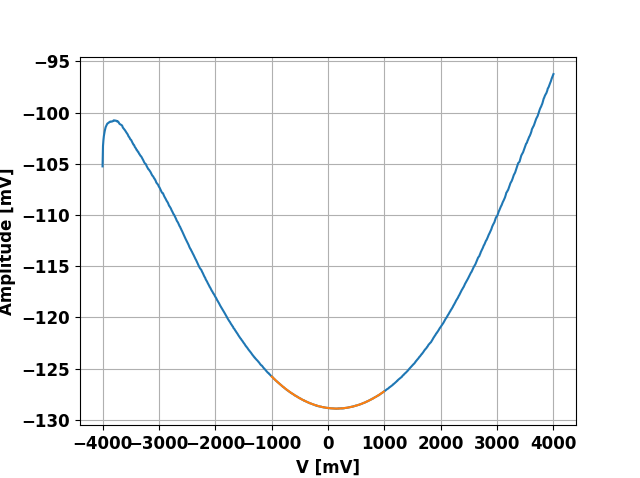
\includegraphics[scale=0.5]{Bilder/Magnetic/amplitude.PNG}
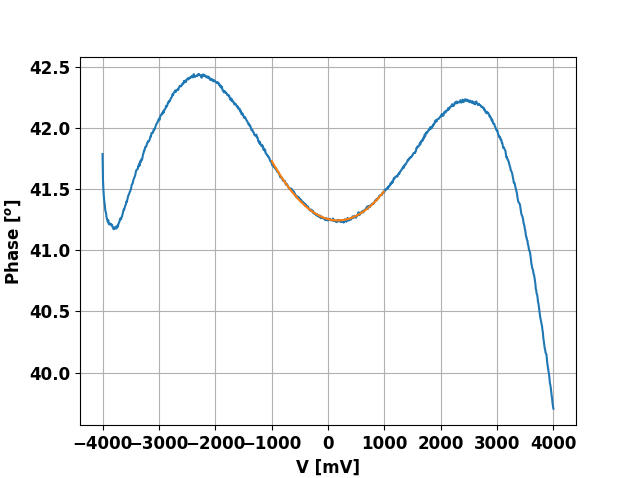
\includegraphics[scale=0.5]{Bilder/Magnetic/phase.PNG}
\caption{Amplitude (top) and Phase (bottom) plotted against the Bias-voltage. A parabolic function is fitted against the extemum in order to extract its offset from 0.}
\label{fig:bias}
\end{figure}

For this a parabolic function is fitted against the data between \SI{-1}{V} and \SI{1}{V}, as seen in figure \ref{fig:bias}. The extremum and its error are directly extracted from this fit. It results in a position of
\begin{equation*}
U_{extr}^{amplitude} = \SI{151.7 \pm 0.3}{mV}
\end{equation*}
\begin{equation*}
U_{extr}^{phase} = \SI{174.8 \pm 1.6}{mV}
\end{equation*}
The weighted mean of the 2 values is
\begin{equation*}
U_{extr}^{mean} = \SI{152.5 \pm 4.2}{mV}
\end{equation*}
which is used to determine the final value of the contact potential difference with the help of equation \ref{eq:phi}:
\begin{equation*}
\Delta\Phi = \SI{152.5 \pm 4.2}{meV}
\end{equation*}


\subsubsection{Domain structure}
as a second part the domain structure of the sample is analyzed. 

%\begin{table}[h]
%\centering
%\begin{tabular}{|c|c|}
%\hline 
%Fabrication technology & "UNIBOND" \\ 
%\hline 
%top Si thickness & \SI{85}{nm} \\ 
%\hline 
%buried oxide thickness & \SI{145}{nm} \\ 
%\hline 
%doping type & p-type (Boron) \\ 
%\hline 
%doping concentration & $1 \times 10^{15}$ \si{\per\cubic\centi\meter} \\ 
%\hline 
%crystal orientation & (100) \\ 
%\hline 
%\end{tabular} 
%\caption{Specification of the SOI wafer.}
%\label{tab:Spec_SOI}
%\end{table}

%\begin{figure}
%\centering
%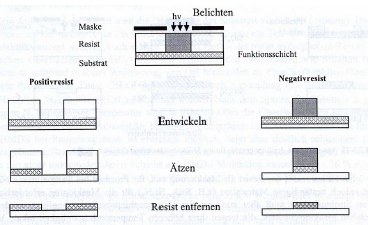
\includegraphics[scale=1.0]{Bilder/Lithographie.PNG}
%\caption{Operating principle of Optical Lithographie with the different steps. Taken from \cite{Volklein00}}
%\label{fig:Lithographie}
%\end{figure}

\bibliography{AFM}% Produces the bibliography via BibTeX.

\end{document}
